\documentclass[../report.tex]{subfiles}
\begin{document}

\section{Discussion} \label{sec:discussion}
\subsection*{Reading from Multiple Addresses}
\begin{wrapfigure}{R}{0.5\textwidth}
    \centering
    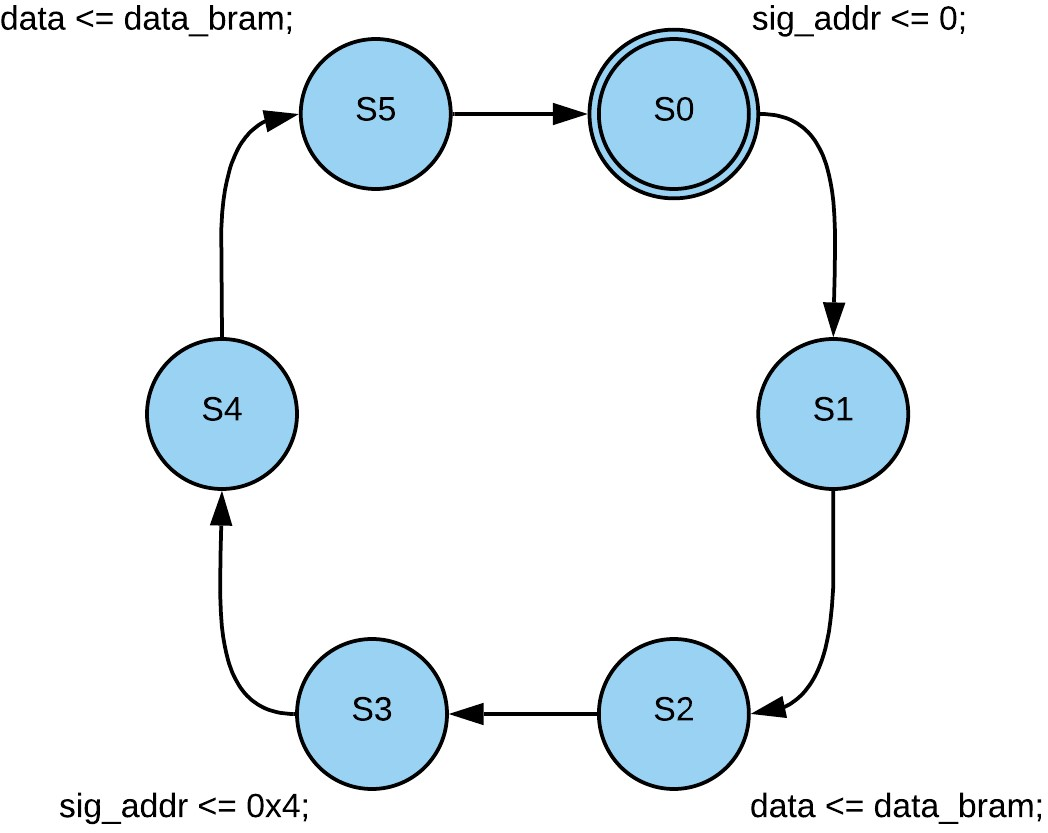
\includegraphics[width=0.5\textwidth]{figures/BRAM_addr_statemachine.jpg}
    \captionsetup{width=0.5\textwidth}
    \caption{A suggested design of a state machine to switch between ram addresses.}
    \label{fig:bram_addr_statemachine}
\end{wrapfigure}

The PWM-value and battery threshold send from the ARM processor to the BRAM described in \autoref{subsec:adc} only uses one address to write the values. If more data was to be send a finites state machine could be designed to switch between addresses of the BRAM on the FPGA. An example of how the state machine could be designed is illustrated in \autoref{fig:bram_addr_statemachine}. 
% \begin{figure}[H]
%     \centering
%     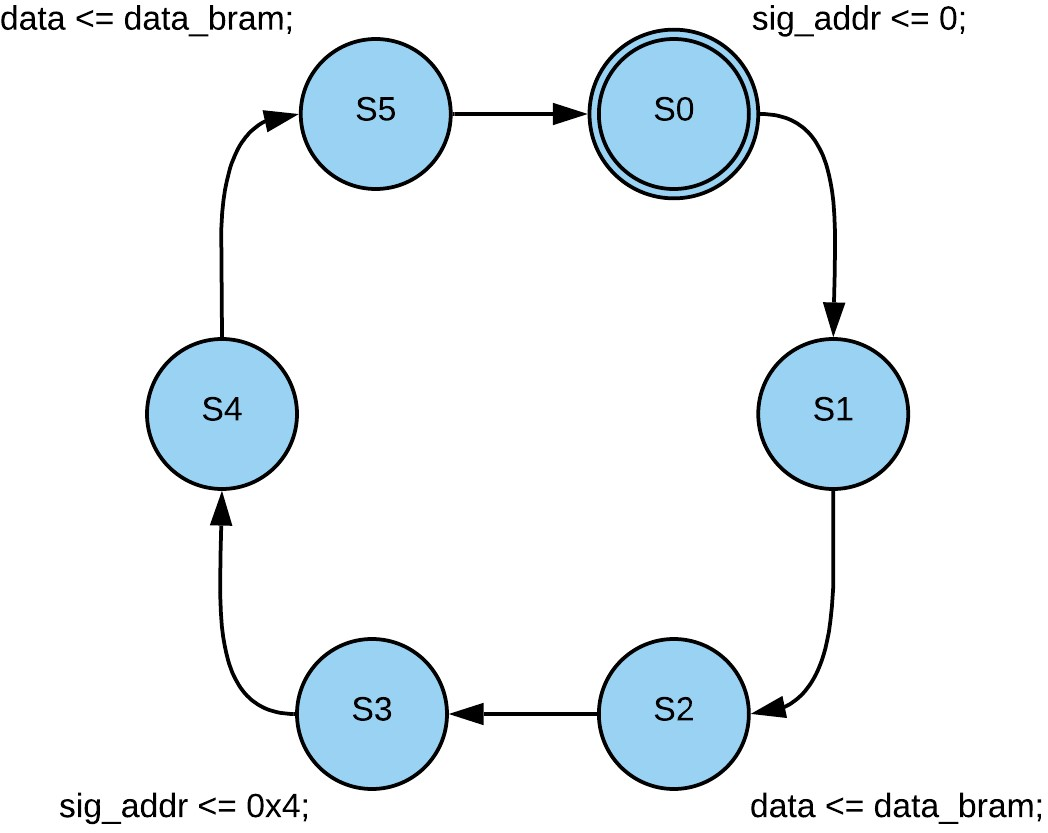
\includegraphics[width=0.75\textwidth]{figures/BRAM_addr_statemachine.jpg}
%     \captionsetup{width=0.75\textwidth}
%     \caption{A suggested design of a state machine to switch between ram addresses.}
%     \label{fig:bram_addr_statemachine}
% \end{figure}

The suggested state machine waits one clock cycle before reading the data from the BRAM since the BRAM reads the address at rising edges and afterwards outputs the data.

\subsection*{Heating of the Inductor}
Initially, the charging circuit was constructed with a single inductor, as shown in \ref{fig:inductors:single}, but this showed to cause problems since it heated drastically.

\begin{figure}[H]
    \centering
    \begin{subfigure}[t]{0.49\textwidth}
        \centering
        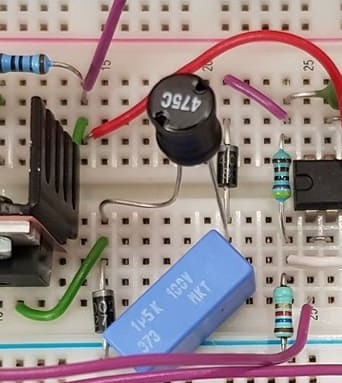
\includegraphics[width=0.9\textwidth]{figures/circuit/single_inductor.jpg}
        \captionsetup{width=0.9\textwidth}
        \caption{The single inductor used in the initial circuit.}  
        \label{fig:inductors:single}
    \end{subfigure}
    \begin{subfigure}[t]{0.49\textwidth}  
        \centering 
        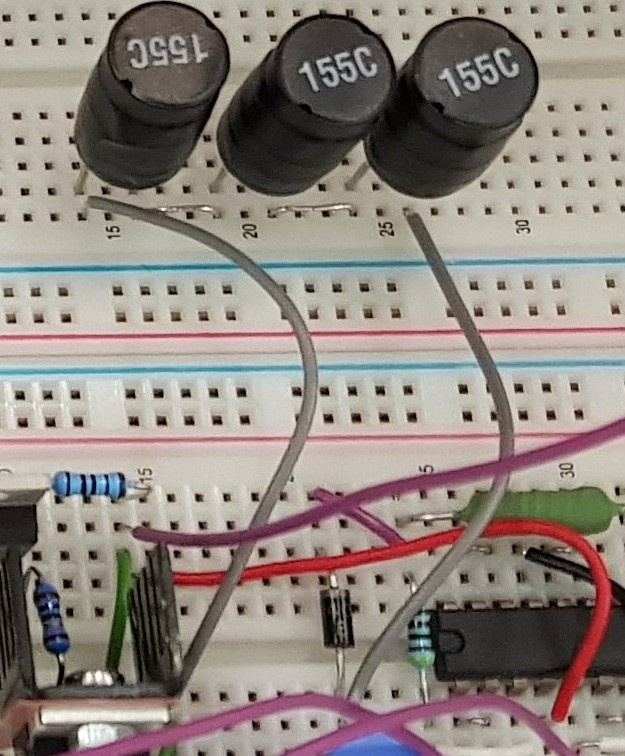
\includegraphics[width=0.9\textwidth]{figures/circuit/triple_inductor.jpg}
        \captionsetup{width=0.9\textwidth}
        \caption{The three inductors used in the final circuit.}  
        \label{fig:inductors:triple}
    \end{subfigure}
    \caption{The inductors used through the development of the circuit.} 
    \label{fig:inductors}
\end{figure}

Therefore, it was chosen to use three inductors in series instead, which summed up to the same size. This distributed the heating between the three components and therefore allowed the circuit to be run for an extended period of time.

\subsection*{Missing Evaluation of 6V Battery}
The circuit was designed to charge batteries up to $6.0 [V]$, but it was not tested in section \ref{sec:results}, since a $6.0 [V]$ battery was not available at the time of testing. Therefore, it is not known if the circuit in practice actually is able to charge a $6.0 [V]$ battery.

\end{document}